\subsubsection{Client}
\setclass{BubbleAndEat::Customer::Client}
\paragraph[::Client]{\class}\mbox{}\\ \label{\class}
\begin{figure}[H]
	\centering
	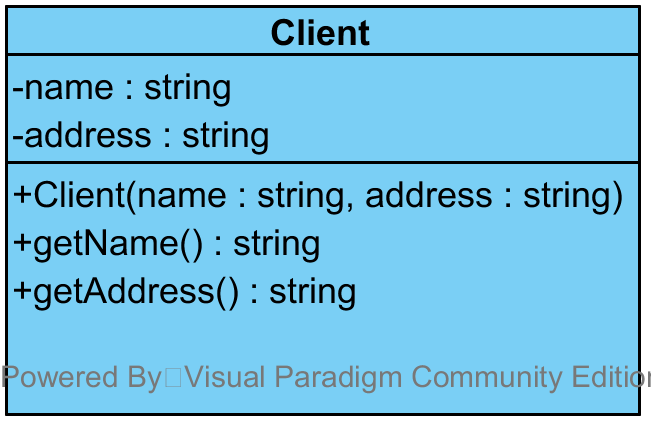
\includegraphics[width=7cm]{./diagrammi/demo/client/customer/client.png}
	\caption{Classe \class}
\end{figure}
\textbf{Descrizione:}\\
Classe che rappresenta un cliente.

\textbf{Utilizzo:}\\
Viene utilizzata per raccogliere le informazioni dei clienti.

%\textbf{Classi ereditate:}
%\begin{itemize}
%	\item \code{}.
%\end{itemize}
%
%\textbf{Sottoclassi:}
%\begin{itemize}
%	\item \coderef{}.
%\end{itemize}

\textbf{Attributi:}
\begin{itemize}
	\item \field{- name: string}: numero cliente;
	\item \field{- address: string}: indirizzo di spedizione.
\end{itemize}

\textbf{Metodi:}
\begin{itemize}
	\item \method{+ Client(name: string, address: string)}: costruttore, assegna i parametri;
	\begin{itemize}
		\item \param{name: string}: nome cliente;
		\item \param{address: string}: indirizzo di spedizione;
	\end{itemize}
	\item \method{+ getName(): string}: ritorna il nome del cliente;
	\item \method{+ getAddress(): string}: ritorna l'indirizzo di spedizione del cliente.
\end{itemize}

\setclass{BubbleAndEat::Customer::CustomerBubble}
\paragraph[::CustomerBubble]{\class}\mbox{}\\ \label{\class}
%\begin{figure}[H]
%	\centering
%	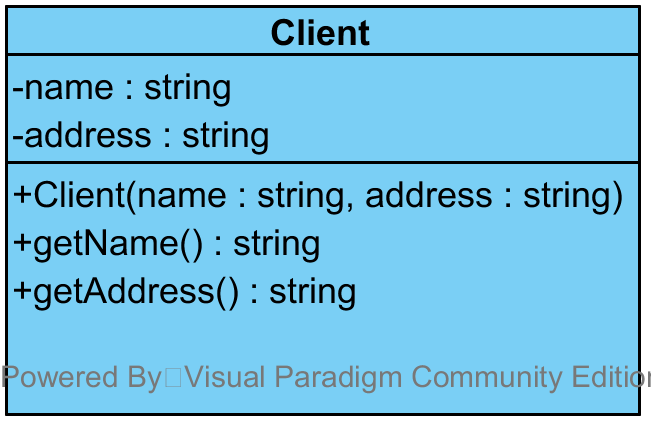
\includegraphics[width=7cm]{./diagrammi/demo/client/customer/client.png}
%	\caption{Classe \class}
%\end{figure}
\textbf{Descrizione:}\\
Classe che rappresenta il Customer e le sue funzionalità all'interno dell'applicazione.

\textbf{Utilizzo:}\\
Viene utilizzata per raccogliere le informazioni dei clienti.

\textbf{Classi ereditate:}
\begin{itemize}
	\item \code{React.Component}.
\end{itemize}

%\textbf{Sottoclassi:}
%\begin{itemize}
%	\item \coderef{}.
%\end{itemize}

\textbf{Attributi:}
\begin{itemize}
	\item \field{-props:Object[]}: array contenente le proprietà degli elementi della lista;
	\item \field{-menu:Menu}: array contenente le diverse entrate del menu;
	\item \field{-page:string}: stringa che indica la pagina corrente;
	\item \field{-quantita:int[]}: array delle quantità dei diversi piatti presenti nell'ordinazione;
	\item \field{-order:Order}: oggetto che rappresenta l'ordine;
	\item \field{-orderState:string} stringa che indica lo stato dell'ordine;
	\item \field{-client:Client}: oggetto che rappresenta il cliente;
	\item \field{-total:int}: numero che indica il totale dei piatti ordinati;
	\item \field{-socket:Socket}: oggetto tramite il quale la classe gestisce la connessione con le altre componenti dell'applicazione;
	\item \field{-orderId}: id dell'ordine del cliente.
\end{itemize}

\textbf{Metodi:}
\begin{itemize}
	\item \method{+ CustomerBubble(props: Object[])}: costruttore, assegna i parametri;
		\begin{itemize}
			\item \param{props: Object[]}: array contenente le proprietà degli elementi.
		\end{itemize}
	\item \method{+ componentDidMount(): void}: viene invocata alla creazione della classe e invoca la funzione connect;
	\item \method{+ componentWillUnmount(): void}: chiama il metodo disconnect alla distruzione della classe;
	\item \method{+ connect():void}: connette la classe al resto dell'applicazione tramite socket;
	\item \method{+ showMenu():void}: invia la richiesta di visualizzazione del menu;
	\item \method{+ order(something:Order):void}: invia l'ordine selezionato;
		\begin{itemize}
			\item \param{something:Order} l'ordine selezionato.
		\end{itemize}
	\item \method{+ queryFor(orderId:string):void}: invia la richiesta di informazioni sullo stato dell'ordine selezionato;
		\begin{itemize}
			\item \param{orderId:string}: id che identifica l'ordine.
		\end{itemize}
	\item \method{+ disconnect():void}: libera le risorse quando viene distrutta la classe;
	\item \method{+ redirectToHome():void}: renderizza e si sposta sulla la pagine home;
	\item \method{+ redirectToMenu():void}: renderizza e si sposta sulla pagina menu;
	\item \method{+ redirectToNewOreder():void}: renderizza e si sposta sulla pagina dei costruzione dell'ordine;
	\item \method{+ rediretToOrder():void}: renderizza e si sposta sulla pagina di gestione dell'ordine; 
	\item \method{+ redirectToInfo():void}: renderizza e si sposta sulla pagina info;
	\item \method{+ reloadTotal():integer}: ricalcola il totale e ne restituisce il valore;
	\item \method{+ addDishToOrder(i:int):void}: invoca updateAmount per aggiungere il piatto selezionato all'ordine;
		\begin{itemize}
			\item \param{i:int}: intero che identifica il piatto.
		\end{itemize}
	\item \method{+ removeDishToOrder(i:int):void}: invoca updateAmount per rimuovere il piatto selezionato dall'ordine;
		\begin{itemize}
			\item \param{i:int}: intero che identifica il piatto.
		\end{itemize}
	\item \method{+ handleChange(e:string,i:int):void}: invoca updateAmount con il valore indicato;
		\begin{itemize}
			\item \param{e:string}: quantità del piatto da aggiungere o rimuovere;
			\item \param{i:int}: intero che identifica il piatto.
		\end{itemize}
	\item \method{+ updateAmount(amount:int,i:int):void}: aggiorna le quantità dei diversi piatti;
	\item \method{+ updateClient(e:string,data:string):void}: aggiorna i dati del cliente;
		\begin{itemize}
			\item \param{e:string}: contiene le nuove informazioni da inserire;
			\item \param{data:string}: indica il tipo di informazione;
		\end{itemize}
	\item \method{+ confirmOrder():void}: effettua l'ordine;
	\item \method{+ render():void}: renderizza il componente.
\end{itemize}
